% Generated with genpdf
% Domain Interno
% Title Norme di Progetto
\documentclass{scalatekids-article}
\begin{document}
\lfoot{Norme di Progetto 0.0.1}
\begin{titlepage}
  \centering
  
\includegraphics[width=0.45\textwidth]{logo.png}\par\vspace{1cm}
  \vspace{1.5cm}
         {\Huge\bfseries Norme di Progetto \par}
         \begin{center}
           \vspace{1.0cm}
                  {\large\bfseries Informazioni sul documento \par}
         \end{center}
         \vspace{-1cm}
         \begin{center}
           \line(1,0){300}
         \end{center}
         \vspace{0cm}
         \begin{tabular}[c]{l|l}
           \textbf{Versione} & 0.0.1\\
           \textbf{Redazione} & Redattore1\\ & Redattore2\\ & Redattore3..\\
           \textbf{Verifica} & Verificatore1\\ & Verificatore2..\\
           \textbf{Responsabile} & Responsabile\\
           \textbf{Uso} & Interno\\
           \textbf{Lista di distribuzione} & ScalateKids
         \end{tabular}
\end{titlepage}
\clearpage
\setcounter{page}{1}
\begin{flushleft}
  \vspace{0cm}
         {\large\bfseries Diario delle modifiche \par}
\end{flushleft}
\vspace{0cm}
\begin{center}
  \begin{tabular}{| l | l | l | l | l |}
    \hline
    Versione & Autore & Ruolo & Data & Descrizione \\
    \hline
    0.0.1 & Andrea Giacomo Baldan & & 2015-12-21 & Creazione scheletro del documento\\
    \hline
  \end{tabular}
\end{center}
\tableofcontents
\section{Sommario}
\prodPurpose
\glossExpl
\section{Comunicazioni}
\subsection{Comunicazioni esterne}
Per le comunicazioni esterne è stata creata una apposita casella di poste elettronica:
\begin{center}
  scalatekids@gmail.com
\end{center}
Questa casella e-mail viene gestita dal \textit{Responsabile di Progetto} che è
colui che si occupa di comunicare con il committente del progetto o con
qualsiasi altra persona esterna al gruppo di lavoro. E' stata impostata per
effettuare l'inolto automatico di tutte le mail in entrata verso gli indirizzi
di tutti i componenti del gruppo, in modo tale che ognuno possa ricevere una
copia della posta in ingresso, tuttavia soltanto il \textit{Responsabile} ha il
potere di inviare posta in uscita.

\subsection{Comunicazioni interne}
\label{sec:Comunicazioni interne}
Per le comunicazioni interne verrà utilizzato un \gloss{forum} apposito su
\textit{Redmine} (vedi sezione \ref{Redmine}), suddiviso in quattro sezioni
principali corrispondenti alle revisioni di avanzamento del progetto:
\begin{itemize}
\item Revisione dei Requisiti
\item Revisione di Progettazione
\item Revisione di Qualifica
\item Revisione di Accettazione
\end{itemize}
Ogni sezione è composta da due sottosezioni, riunioni e comunicazioni, le quali
conterranno rispettivamente le riunioni indette, seguite dalla disponibilità dei
membri a partecipare e, a seguito di avvenuta riunione, il riassunto dei punti
discussi e le comunicazioni di carattere più o meno generale riguardanti
attività della revisione di appartenenza.\\ Ogni \gloss{topic} all'interno di
queste due sottosezioni dovrà rispettare il seguente formato:
\begin{itemize}
\item\textbf{Riunioni:}\\
  \textit{Riunione Dominio - Data AAAA-mm-dd - Oggetto}\\
  (es: Riunione Interna - 2015-12-29 - Strategie Ciclo di Vita)
\item\textbf{Comunicazioni:}\\
  \textit{Oggetto - Data}\\
  (es: Design Pattern - 2016-01-12)
\end{itemize}
La voce \textit{Oggetto} dovrà essere esplicativa del contenuto, più possibile
stringata e non confondibile con precedenti \gloss{topic}. E' ammesso
l'inserimento di allegati purchè strettamente pertinenti al \gloss{topic}, ad
esempio il verbale di una riunione o il riassunto di qualche discussione
avvenuta al di fuori delle riunioni.\\
Vengono usati altri strumenti ufficiosi per lo scambio di informazioni:
\begin{itemize}
\item applicazioni di \gloss{instant messaging} quali \textit{Whatsapp} e il suo servizio \textit{Whatsapp Web};
\item applicazioni \gloss{VoIP} per effettuare audio conferenze con un qualsiasi numero di componenti, quale \textit{TeamSpeak3};
\item servizi online per la gestione di una \gloss{whiteboard} condivisa, quale \textit{Twiddla};
\end{itemize}
Abbiamo deciso che qualora membri del gruppo si scambino informazioni attraverso
questi strumenti sopra elencati dovranno, se presenti informazioni di interesse
per il progetto, mandare un sunto della suddetta conversazione sul \gloss{forum}
per tenere informati tutti i membri del gruppo sullo stato di avanzamento nella
sottosezione comunicazioni.\\ Solo in caso di necessità derivate dalla mancanza
di infrastrutture (es. collegamento a internet) si potrà comunicare attraverso
SMS o chiamate telefoniche, anche in questo caso si dovrà verbalizzare quanto
detto attraverso il \gloss{forum} appena possibile.

\section{Riunioni}

\subsection{Riunioni Interne}
Tutti i componenti del gruppo possono avanzare una richiesta per una riunione
interna seguendo le regole per la richiesta (vedi \ref{Regole per la
  richiesta}).\\ Sarà il \textit{Responsabile di Progetto} a decidere se indire
o meno questa riunione, controllando la disponibilità dei membri attraverso il
forum e in caso avvertendo tutti attraverso un \gloss{topic} come spiegato in
sezione \ref{Comunicazioni}.\\ E' richiesta la partecipazione di almeno 4 membri
del gruppo.

In casi particolari, come per riunioni che trattano specifici ambiti non di
interesse di tutti i membri o per l'avvicinarsi a importanti date, si può indire
una riunione di gruppo con meno compomenti presenti, sempre tramite
l'approvazione del \textit{Responsabile}.

\subsection{Riunioni esterne}
Le riunioni esterne (incontri col committente o proponente) possono essere
proposte da qualunque membro del gruppo, spetta sempre al \textit{Responsabile
  di Progetto} la decisione finale.\\ E' necessaria la presenza di almeno il
50\% + 1 dei componenti.

\subsection{Regole per la richiesta}
Le richieste vanno effettuate tramite mail al responsabile e devono avere come oggetto:
\begin{center}
  Richiesta riunione <tipo riunione>
\end{center}
tipo riunione può essere interna o esterna.
Il corpo della mail dovrà avere una struttura del tipo:
\begin{center}
  Motivazione: <motivo riunione>
  Data proposta: <data>
  Luogo proposto: <luogo>
\end{center}

\subsection{Esiti Riunioni}
Ad ogni riunione verrà dato il compito a uno dei presenti di verbalizzare un riassunto sugli argomenti trattati e i chiarimenti esermi durante tale riunione.\\
Questa persona avrà poi l'obbligo di condividere il verbale con tutti i componenti sul \textit{Drive} del gruppo e di notificare l'avvenuto caricamento tramite \textit{forum}

\section{Documenti}
% TODO: bisogna aggiungere la parte in cui diciamo che usiamo una virtualbox per facilitare tutto

\subsection{Struttura dei documenti}
Abbiamo standardizzato la scrittura di tutti i documenti attraverso un \gloss{template} \LaTeX\xspace creato da noi e presente su \textit{github} nel \gloss{repository} \textit{ActorBase - Documents}.\\
L'uso del template ci permette di creare una serie di documenti stilisticamente uniformi tra loro e ci facilita la modifica delle parti in comune tra essi.\\
Il template regola:
\begin{itemize}
\item Formattazione dei documenti (font)
\item Formattazione delle pagine (header e footer pagine)
\item Raggruppa tutti i pacchetti utilizzati
\item Aggiunge comandi personalizzati
\item Collegamenti tra indice e categorie o sezioni
\end{itemize}
% TODO: rivedere cosa regola il template

Ogni documento presenta in ordine:
\begin{itemize}
\item Diario delle modifiche: è una tabella in cui sono scritte le diverse modifiche fatte dai membri sul documento;
\item Indice: indice con collegamenti alle categorie e alle sezioni del documento;
\item Introduzione: contiene alcune sottosezioni:
  \begin{itemize}
  \item Scopo del documento;
  \item Glossario;
  \item Riferimenti inerenti al documento in questione;
  \end{itemize}
\item Resto del documento: contenuto specifico;
\end{itemize}

Abbiamo creato uno script \textit{perl} per la creazione automatica dello scheletro di un generico documento.

\subsection{Struttura Pagina}
L'intestazione di ogni pagina contiene:
\begin{itemize}
\item Logo gruppo;
\item Nome gruppo;
\item Sezione corrente del documento;
\end{itemize}
Il piè pagina invece contiene:
\begin{itemize}
\item Nome documento;
\item Pagina corrente rispetto al numero di pagine totali;
\end{itemize}

\subsection{Norme tipografiche}
Per uniformare il più possibile la stesura di tutti i documenti abbiamo scelto delle regole che tutto il gruppo deve seguire.

\subsubsection{Punteggiatura}
\begin{itemize}
\item \textbf{Punteggiatura}: tutti i segni di punteggiatura devono essere seguiti da uno spazio e non avere spazi precedenti al segno stesso;
\item \textbf{Maiuscole}: le lettere maiuscole devono essere usate dove previsto dalla lingua italiana.
  Saranno inoltre scritti con l'iniziale maiuscolta i ruoli, le persone inerenti al progetto e i documenti noti (es. \textit{Committente} \textit{Analisi dei Requisiti});
\end{itemize}

\subsubsection{Stile testo}:
\begin{itemize}
\item \textbf{Corsivo}: il corsivo dev'essere utilizzato per:
  \begin{itemize}
  \item Abbreviazioni;
  \item Citazioni;
  \item Documenti (es \textit{Analisi dei Requisiti});
  \item Porre un enfasi maggiore alla parola e/o frase;
  \end{itemize}
\item \textbf{Grassetto}: il grassetto dev'essere usato per:
  \begin{itemize}
  \item Evidenziare passaggi o concetti importanti;
  \item Sezioni e sottosezioni dei documenti;
  \end{itemize}
\item \textbf{Maiuscolo}: alcuni acronimi saranno scritti interamente in maiuscolo (es. \textit{SQL});
\item \textbf{Monospace}: i font monospace saranno usati per riportare parti di codice;
\end{itemize}

\subsection{Formati di riferimento}
\begin{itemize}
\item \textbf{Riferimenti}:
  \begin{itemize}
  \item Percorsi web: per gli indirizzi web e per gli inidirizzi e-mail deve essere usato il comando \LaTeX\xspace
    \begin{center}
      \verb=\url{percorso}=
    \end{center}
  \item Link ad altri PDF:
    \begin{center}
      \verb=\href{run:<pathToPDF>/<namefile.pdf>}{<name of the link>}=
    \end{center}
  \item Link a sezioni interne al documento: per link a sezioni interne al documento corrente deve essere utilizzato il documento \LaTeX\xspace
    \begin{center}
      \verb=\ref{riferimento a sezione}=
    \end{center}
  \end{itemize}
\item \textbf{Date}: Le date devono essere espresse seguento lo standard \textit{\gloss{ISO}} 8601:2004:
  AAAA-MM-GG
  AAAA: rappresenta l'anno (es. 2015);
  MM:	rappresenta il mese (es. 12);
  GG: rappresenta il giorno (es. 21);

\item \textbf{Abbreviazioni}: per semplicità possono essere abbreviati i nomi dei seguenti documenti:
  AR: \textit{Analisi dei Requisiti}
  RR: \textit{Revisione dei Requisiti}
  GL: \textit{Glossario}
  NP: \textit{Norme di Progetto}
  RP: \textit{Revisione di Progettazione}
  PQ: \textit{Piano di Qualifica}
  RQ: \textit{Revisione di Qualifica}
  PP: \textit{Piano di Progetto}
  SF: \textit{Studio di Fattibilità}
  RA: \textit{Revisione di Accettazione}

\item \textbf{Nomi ricorrenti}:
  \begin{itemize}
  \item Ruoli: come già scritto in precedenza i ruoli di progetto devono essere scritti con la prima lettera di ogni parola maiuscola ed in corsivo, escludendo le proposizioni (es. \textit{Responsabile di Progetto});
  \item Nomi dei files: i nomi dei files relativi a documenti devono seguire
    la notazione \textit{\gloss{CamelCase}}, seguiti da \textit{\_v} e dalla
    versione del file (es. NormeDiProgetto\_v1.0.1.pdf);
  \item Nome del progetto: sarà indicato come \textbf{Actorbase};
  \item Nome del committente: il committente sarà indicato come \textit{prof. Tullio Vardanega};
  \item Nome del proponente: il proponente sarà indicato come \textit{prof. Riccardo Cardin};
  \item Nome del gruppo: il gruppo sarà indicato come \textit{ScalateKids}.
  \end{itemize}
\end{itemize}

\subsection{Tabelle}
% TODO: mettiamo tabelle? se si decidere come uniformarle

\subsection{Immagini}
Utilizziamo immagini con formato \textit{JPG} o \textit{PNG}, questi ultimi rendono immediata l'inculsione delle suddette immagini nei documenti.

\subsection{Integrazione termini di lingua straniera}
Per non incorrere in diverse modalità di integrazione per l'uso di vari termini di lingua straniera (es. file, repository ecc...) abbiamo deciso di non pluralizzare i termini non italiani, esempi:\\
abbiamo utilizzato delle \textit{repository} per... (non \textit{repositories}).
Questa scelta è derivata da una ricerca che ha fornito diverse fonti riguardanti l'uso di questa norma nell'uso della lingua italiana, il sottostante sito web raccoglie diverse fonti trovate:\\
\begin{center}
  \url{http://www.darsch.it/?pg=sphere&postid=954}
\end{center}

\subsection{Versionamento documenti}
La documentazione prodotta deve avere un numero di versione avente la seguente struttura:\\
\begin{center}
  vX.Y.Z
\end{center}
in cui:
\begin{itemize}
\item \textbf{X}: aumenta con il numero di uscite formali del documento;
\item \textbf{Y}: rappresenta il numero di modifiche sostanziali effettuate sul documento. Se pari a 0 indica che il documento è ancora in fase di stesura in presente revisione;
\item \textbf{Z}: rappresenta il numero di modifiche minori effettuate sul documento.
\end{itemize}
 % TODO: spiegare come aumentano ste versioni

\subsection{Ciclo di vita dei documenti}
Tutti i documenti nascono nello stato di \textit{in lavorazione}.\\
Dopo l'avvenuta di tute le modifiche necessarie per arrivare ad una versione completa del documento, il suddetto si verrà a trovare nello stato \textit{da verificare}.\\
Alla fine della fase di verifica del documento, se approvato il documento andrà nello stato di \textit{approvato}.
I tre stati sono descritti brevemente come segue:
\begin{itemize}
\item \textbf{In lavorazione}: il documento nasce in questo stato e ci rimane fino a che non è avvenuta una sua completa stesura;
\item \textbf{Da verificare}: il documento resta in questo stato finchè i \textit{Verificatori} assegnati ad esso non effettueranno un controllo atto a trovare e a correggere errori di ogni tipo;
\item \textbf{Approvato}: dopo la fase di verifica il \textit{Responsabile} effettuerà una fase di approvazione, se questa fase sarà superata il documento sarà approvato e entrerà in una versione ufficiale.
\end{itemize}

\subsection{Norme di verifica documenti}
Posto che tutti i componenti del gruppo dovranno affettuare delle attività di
verifica, il redattore di ogni sezione nei documenti tassativamente non potrà
effettuare verifica e approvazione delle parti redatte dallo stesso,
coerentemente con le strategie scelte nel \textbf{PQ}.

\section{Norme di codifica dei file}
\subsection{Codifica}
Tutti i file contenenti codice o documentazione dovranni essere conformi alla
codifica \gloss{UTF-8}.
\subsection{Linee guida stilistiche}
La stesura del codice dovrà seguire pedissequamente alcune regole al fine di
garantire un buon livello di manutenibilità e verificabilità del prodotto, in
particolare gli sviluppatori dovranno attenersi alle \textit{Scala Style Guide}
(\url{https://docs.scala-lang.org/style/}), in particolar modo non possono
essere infrante le seguenti regole:
\begin{itemize}
  \item Lunghezza massima linee 80 caratteri;
  \item Identazione di 2 spazi;
  \item Posizionamento di parentesi graffe in linea con il blocco struttura di
    riferimento;
\end{itemize}
Tutti i file contenenti codice dovranno essere redatti in lingua inglese.
\subsubsection{Nomenclatura}
I nomi di variabili, metodi e funzioni seguiranno la convenzione
\textit{\gloss{lowerCamelCase}}, i nomi di classi invece
\textit{\gloss{UpperCamelCase}}.
\subsubsection{Ricorsione}
La ricorsione va evitata il più possibile, per ogni funzione ricorsiva sarà
necessario fornire una prova di terminazione e il costo in memoria. L'utilizzo
deve giustificare la spesa in termini di memoria rispetto al risparmio in
termini di istruzioni.
\subsubsection{Documentazione}
% TODO: Cardin: Licenza sull'intestazione di tutti i file?
I file contenenti codice dovranno seguire le linee guida \gloss{scaladoc}
\url{https://docs.scala-lang.org/style/scaladoc.html} ed essere provvisti di un
intestazione contenente:
\begin{lstlisting}
  /**
   * Nome file
   * Breve descrizione
   *
   * @author Autore del file
   * @version Versione
   * @date Data di creazione
   * Descrizione dettagliata del file
   */
\end{lstlisting}
Prima di ogni metodo dovrà essere presente un commento \gloss{scaladoc} contenente:
\begin{lstlisting}
  /**
   * Breve descrizione del metodo
   *
   * @param Nome del primo parametro
   * @param Nome del secondo parametro
   * @return Valore di ritorno del metodo
   * @throws Eccezioni lanciate dal metodo
   */
\end{lstlisting}
La documentazione verrà generate da \gloss{scaladoc}, nel caso si verifichi la
necessità di documentare del codice di difficile comprensione, sarà possibile
inserire un commento nelle righe precedenti, dopo aver verificato
l'impossibilità di effettuare un \gloss{refactoring}.

\section{Requisiti di Progetto}
\subsection{Classificazione}
I requisiti dovranno essere classificati per tipo e importanza.

\section{Ruoli di progetto}
Durante l'intera fase di sviluppo del progetto, dalla formazione del gruppo alla
Revisione di Accettazione vi saranno alcuni ruoli ben precisi da ricoprire. Si
tratta di funzioni aziendali assegnate a progetto, specializzate in campi ben
specifici all'interno dell'azienda. Tra questi ruoli, alcuni avranno maggior
presenza in determinate fasi del progetto rispetto ad altre, dove addirittura
potrebbero non figurare definitivamente, ma tutti sono essenziali per il buon
esito del progetto.\\ Ciascun componente dovrà ricoprire almeno una volta ogni
ruolo, sarà inoltre possibile ricoprire più ruoli, sia contemporaneamente che in
distinte fasi del progetto, purchè sia garantita l'assenza di conflitti
d'interesse nello svolgimento di attività di verifica e approvazione.
\subsection{Responsabile di Progetto}
Il \textit{Responsabile di Progetto} rappresenta il progetto presso il fornitore
e presso il committente, è il ruolo più presente lungo tutto l'arco temporale di
sviluppo del prodotto in assoluto, in quanto deve partecipare e seguire la
crescita fino al rilascio del prodotto. Deve avere conoscenze e capacità
tecniche in modo da comprendere e anticipare l'evoluzione del progetto.\\
Detiene il potere decisionale e ha resposabilità su:
\begin{itemize}
  \item Pianificazione;
  \item Gestione delle risorse umane;
  \item Controllo, coordinamento e relazioni esterne;
  \item Analisi e gestione dei rischi;
  \item Approvazione dei documenti;
  \item Approvazione dell'offerta economica;
\end{itemize}
Si occupa dunque della distribuzione delle attività, verifica che esse vengano
portate a termine seguendo le \textit{Norme di Progetto} e controlla che non vi
siano conflitti d'interesse tra redazione e verifica, ha il compito inoltre di
risolvere eventuali situazioni critiche tra i componenti del gruppo qualora
sorgessero conflitti.\\ Redige il \textit{Piano di Progetto} e collabora alla
stesura del \textit{Piano di Qualifica}.
\subsection{Analista}
L'\textit{Analista} è una figura molto presente nelle prime fasi del progetto e
determina fortemente la buona riuscita del prodotto. Non si occupa della
soluzione al problema ma deve offrire una specifica di progetto che comprenda
appieno la natura e la complessità del problema, che possa essere in seguito
valutata dal \textit{Progettista} al fine di fornire una soluzione.\\ Redige lo
\textit{Studio di Fattibilità} e l'\textit{Analisi dei Requisiti}, partecipa
inoltre alla stesura del \textit{Piano di Qualifica}.
\subsection{Amministratore}
L'\textit{Amministratore} si occupa di allestire, seguire e migliorare
l'ambiente di lavoro, le responsabilità principali sono:
\begin{itemize}
  \item Amministrazione delle risorse e delle infrastrutture;
  \item Risoluzione di problemi legati alla gestione dei processi;
  \item Gestione della documentazione di progetto;
  \item Controllo di versioni e configurazioni;
  \item Ricerca di strumenti che possano automatizzare compiti tediosi;
  \item Ricerca di strumenti che possano semplificare il lavoro di verifica;
\end{itemize}
Redige le \textit{Norme di Progetto} e partecipa alla stesura del \textit{Piano
  di Qualifica}.
\subsection{Progettista}
Il \textit{Progettista} è una figura molto legata all'\textit{Analista}, in
quanto è responsabile delle attività di progettazione, si occupa dunque di
trovare una soluzione efficace al problema, sfruttando le proprie competenze
tecniche e tecnologiche sempre aggiornate. Si tratta di un ruolo generalmente
presente dalla fase di progettazione fino alla fine del progetto.
\subsection{Programmatore}
E' responsabile delle attività di codifica e manutenzione del prodotto, gestisce
inoltre le componenti di ausilio necessarie all'attività di verifica e
validazione. Hanno competenze tecniche specializzate, ricoprono principalmente
le seguenti responsabilità:
\begin{itemize}
  \item Implementazione delle soluzioni descritte dal \textit{Progettista}
    seguendone i design pattern proposti;
  \item Documentare e commentare il codice in modo da renderlo più facilmente
    manutenibile;
  \item Implementare dei test utili in fase di verifica e validazione;
\end{itemize}
Si occupa della redazione del \textit{Manuale Utente}.
\subsection{Verificatore}
La figura del \textit{Verificatore} partecipa alla realizzazione del prodotto per
tutta la durata assieme al \textit{Responsabile}, possiede grandi capacità di
giudizio e competenza tecnica, influenza molto fortemente l'aspetto qualitativo
del prodotto.\\ Ricopre le seguenti responsabilità:
\begin{itemize}
  \item Si assicura che le attività seguano le direttive stabilite nelle \textit{Norme di Progetto};
  \item Controlla la conformità di ogni stadio del ciclo di vita del prodotto.
\end{itemize}
Si occupa della redazione del \textit{Piano di Qualifica}.
\section{Glossario}
Il glossario è un documento unico per tutti i documenti, esso conterrà tutte le
definizioni, in ordine lessicografico crescente, dei termini inerenti al tema
del progetto o che possono essere fraintesi. I termini che dovranno essere
inseriti nel glossario saranno contrassegnati da una G pedice all'interno dei
documenti. Prima di inserire un nuovo termine bisogna assicurarsi che non sia
già presente.\\ Il comando \LaTeX\xspace da utilizzare per contrassegnare un
termine da glossario all'interno dei documenti è \verb=\gloss=, mentre l'inserimento
di una nuova parola all'interno del glossario è \verb=\glossDef=. La scelta di creare
un comando apposito per un operazione ``elementare'' è scaturita
dall'agevolazione che porta alla stesura della documentazione: avendo un modo
univoco di riconoscere i termini all'interno del glossario, è possibile
automatizzare il controllo delle parole da glossario all'interno dei
documenti(vedi sezione \ref{sec:script}).

\section{Ambiente di lavoro}
\subsection{Apparato di collaborazione}
Per coordinare il lavoro tra i componenti del gruppo, trovandosi spesso a dover
operare in remoto, l'azienda ha scelto di utilizzare quanto più possibile gli
strumenti di condivisione e versionamento erogati come servizi web,
centralizzando gli strumenti organizzativi su server privato.
\subsubsection{Servizi web}
I servizi web utilizzati sono:
\begin{itemize}
\item\textbf{Google Drive:} è usato per lo scambio di file e documenti all'interno del gruppo, principalmente per file che non necessitano di versionamento.\\
  Questo spazio del gruppo è suddiviso in diverse cartelle per una migliore gestione e per facilitare la ricerca all'interno di esso.\\
  Il \textit{Responsabile di Progetto} ha il potere amministrativo dell'account in questione, quindi sarà quest'ultima persona ad occuparsi di garantire i giusti diritti ai membri del gruppo.
\item\textbf{Github:} è usato per tutti i files che necessitano un sistema di \gloss{versionamento} viene usato il servizio offerto da \textit{Github}, l'indirizzo web del gruppo è:\\
  \begin{center}
    \url{https://github.com/scalatekids}
  \end{center}
\item\textbf{Twiddla:} è un sistema che offre una lavagna online condivisa, questo servizio è utilizzato dai membri del gruppo per discutere e lavorare assieme % TODO: non so cosa scrivere su twiddla
\item\textbf{Gantter for Google Drive:} è uno strumento gratuito per la creazione di \gloss{diagrammi di Gantt}, è stato usato per la creazione del Gantt predittivo
\end{itemize}
\subsubsection{Server dedicato}
Sono state installate alcune applicazioni per il coordinamento del gruppo su
server dedicato, gestito dall'\textit{Amministratore} su direttive del
\textit{Responsabile}.\\ Il server è raggiungibile da interfaccia web previo
login, i componenti possono usufruire delle seguenti applicazioni:

\paragraph{Redmine}
Redmine è un'applicazione web atta alla gestione di progetti.\\
Offre diverse funzionalità che il gruppo dovrà utilizzare, quali:
\begin{itemize}
\item\textbf{Sezione wiki:} una pagina web in cui il gruppo andrà a condividere una serie di link di interesse riguardanti ogni tecnologia o aspetto inerente al progetto.
\item\textbf{Sistema di segnalazioni:} un sistema di segnalazioni gestite dall'\textit{Responsabile}, ogni segnalazione rappresenta un task assegnato ad uno o più membri del gruppo, il suo conseguimento servirà per il soddisfacimento di un requisito.
\item\textbf{Gantt:} \textit{Redmine} costruisce automaticamente un \gloss{diagramma di Gantt} con le segnalazioni create dall'\textit{Responsabile}
\end{itemize}
% TODO: potremmo aggiungere dei diagrammi UML2.0 per descrivere come usare redmine...

\paragraph{PHPMyAdmin}
PHPMyAdmin è uno strumento scritto in linguaggio \textit{PHP} che offre una facile amministrazione di \gloss{\textit{database}}.\\
Questo strumento verrà usato per la creazione di un back-end per la gestione dei requisiti.	% TODO: scrivere qualcosa di più a riguardo?
% TODO: da integrare se aggiungiamo il front-end

\subsubsection{Versionamento}
Lo strumento scelto è \gloss{git} principalmente per la grande diffusione negli
ambienti di sviluppo e per l'integrazione offerta dal servizio web
\textit{Github}, il quale è inoltre offre un esaustiva documentazione
sull'utilizzo del programma in questione. Infine \gloss{git} si è rivelato essere
il più conosciuto tra i membri del gruppo, l'alternativa \gloss{SVN}, nonostante
i simili principi di funzionamento, costituiva una scelta più difficoltosa, in
quanto nessun membro ha mai avuto esperienze di utilizzo.
Sono stati creati due \gloss{repository} all'indirizzo \url{https://github.com/scalatekids}:
\begin{itemize}
\item Actorbase.\gloss{git}: Contiene i sorgenti del software.
\item Actorbase-Documents.\gloss{git}: Contiene i sorgenti \LaTeX\ e i PDF generati.
\end{itemize}

\subsubsection{Ambiente di lavoro individuale}
Per il lavoro individuale, è stato pensato ad un modo di uniformare quanto più
possibile l'ambiente di sviluppo tra i componenti; il \textit{Responsabile} e
l'\textit{Amministratore} hanno stabilito l'\gloss{IDE} di base ed è stata creato
un ambiente virtuale comune utilizzando il software \textit{Virtualbox}. Tutti i
componenti del gruppo utilizzeranno gli strumenti all'interno della
\gloss{virtual machine} in modo da garantire omogeneità, e riproducibilità di
eventuali \gloss{bug}.\\ L'\textit{IDE} scelto è \textit{IntelliJIdea}, considerato il
più appropriato e compatibile con le tecnologie centrali del progetto, gli
editor \textit{vim}, \textit{emacs} o \textit{Sublime Text 2} potranno essere
utilizzati dai componenti del gruppo, purchè si tratti di modifiche rapide o
stesura di script di utilità generale.\\
Per la stesura dei documenti, l'\gloss{IDE} di riferimento è \textit{TeXstudio}.
\paragraph{Installazione virtual machine}
Una volta ottenuto il file \textit{.vdi} presente sul \textit{Drive} del gruppo
in forma compattata \textit{.7z}, ogni componente dovrà installare il software
\textit{Virtualbox} sul proprio computer e procedere con la creazione della
macchina virtuale.\\
I passi da seguire sono:
\begin{itemize}
  \item Nuovo
  \item Tipo: \textit{Ubuntu} Versione: \textit{64-bit}
  \item Assegnare la quantità di memoria in base alla propria disponibilità
  \item Usa un hard-disk esistente e selezionare \textit{ScalateKids-VMvX.Y.vdi}
\end{itemize}
Una volta avviata la macchina, da terminale lanciare il comando:
\begin{center}
  \textit{curl http://codep.kissr.com/sk/scripts/init.sh | sh}
\end{center}
Il comando provvederà al download delle librerie e degli \gloss{script}
necessari alla corretta configurazione dell'ambiente di lavoro del gruppo.
Al termine la macchina virtuale sarà pronta ad essere utilizzata per lo sviluppo.
\paragraph{Versionamento virtual machine}
Di volta in volta, lungo tutto l'arco del progetto, quando sarà necessario
modificare l'ambiente di lavoro o ci sarà bisogno di librerie di supporto
ulteriori o modifica di \gloss{script} di utilità, il seguente comando si
occuperà di scaricare e installare gli aggiornamenti richiesti:
\begin{center}
  \textit{curl http://codep.kissr.com/sk/scripts/update.sh | sh}
\end{center}
Gli \gloss{script} init.sh e update.sh presenti sul server privato saranno
preparati dall'\textit{Amministratore} e rilasciati di volta in volta previa
approvazione del \textit{Responsabile}.
\paragraph{Script di utilità locali}
\label{sec:script}
L'\textit{Amministratore} si è occupato di scrivere alcuni \gloss{script} di utilità
generale da utilizzare all'interno della macchina virtuale:
\begin{itemize}
  \item\textbf{gencln:} lanciato senza argomenti, genera tutti i pdf del
    progetto dai .tex, eliminando tutti i file .log .aux .out .soc e .toc
    generati. Può avere un numero indefinito di argomenti, purchè siano file
    .tex, questi verranno allo stesso modo generati eliminando tutti i file .log
    .aux .out .soc e .toc
  \item\textbf{extgloss:} estrae tutti i termini da glossario contrassegnati da
    \verb=\gloss= dai file del progetto, anche questo comando può essere lanciato con
    o senza argomenti
  \item\textbf{checkgloss:} genera una lista di file da glossario leggendo il
    file \hyperref{Glossario\_v0.0.1}, in seguito controlla tutti i file del
    progetto eccetto il glossario, e inserisce il comando \verb=\gloss= sui termini
    contenuti in lista trovati nei file. Con argomenti esegue le medesime
    operazioni soltato sui file .tex scelti.
\end{itemize}
\paragraph{Script di utilità remoti}
Questi script, \textbf{init.sh} e \textbf{update.sh}, risiederanno sul server
privato, e avranno rispettivamente lo scopo esclusivo di inizializzare e
aggiornare l'ambiente di lavoro della virtual machine.
% TODO: manca il software che utilizziamo per fare gli uml, e dirgli che versione di uml usiamo
come standard

\section{Redmine}
Questo capitolo è un tutorial su come usare correttamente \textit{Redmine}.
Questo software offre una vasta gamma di servizi molto utili per la gestione di un progetto, noi in particolare useremo il \textit{forum}, la sezione wiki ed il sistema di segnalazioni che automaticamente costruisce il diagramma di \textit{Gantt}. Tramite installazioni di \gloss{plugin} è possibile aggiungere funzionalità. Se un componente del gruppo ritenga necessaria l'installazione di un \gloss{plugin}, costui può proporla al \textit{Responsabile di Progetto} il quale affiderà il compito ad un \textit{Amministratore} se la riterrà una funzionalità utile.
\subsection{Creare un sottoprogetto}
La creazione di sottoprogetti è molto utile per mantenera una chiara divisione funzionale tra le attività, la creazione di un sottoprogetto è molto semplice come si vede in figura sottostante
\begin{figure}[H]
  \centering
  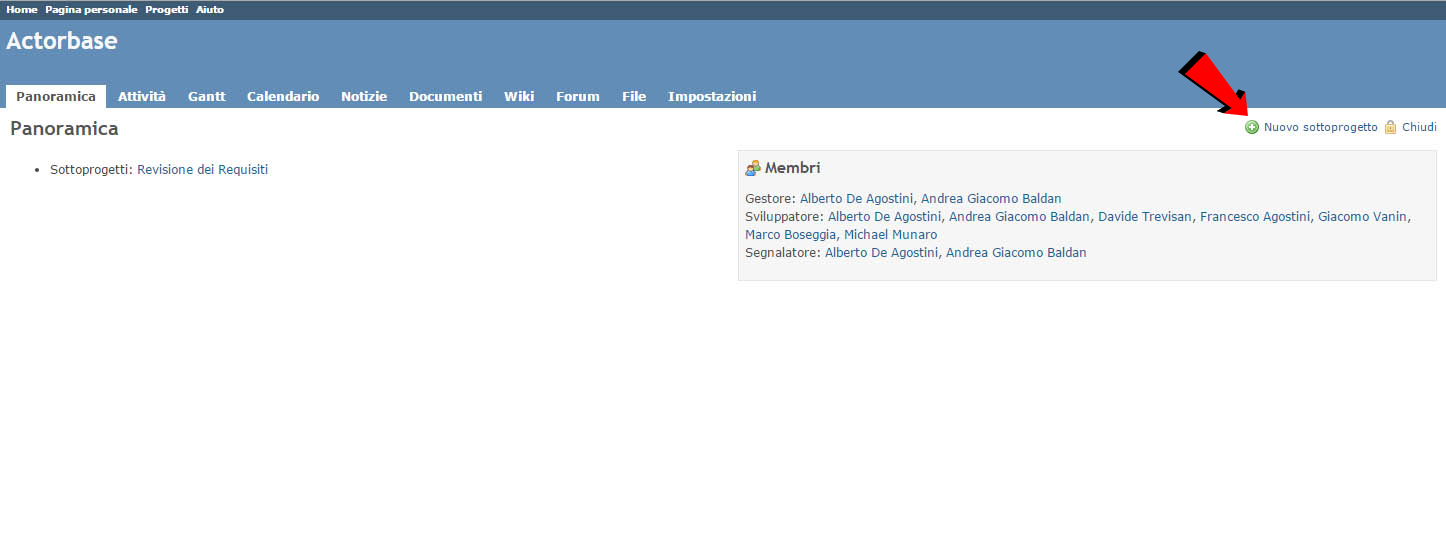
\includegraphics[width=1\textwidth]{tutorialsRedmine/creaproj1.png}
  \caption{come creare un sottoprogetto - figura 1}
\end{figure}
\begin{figure}[H]
  \centering
  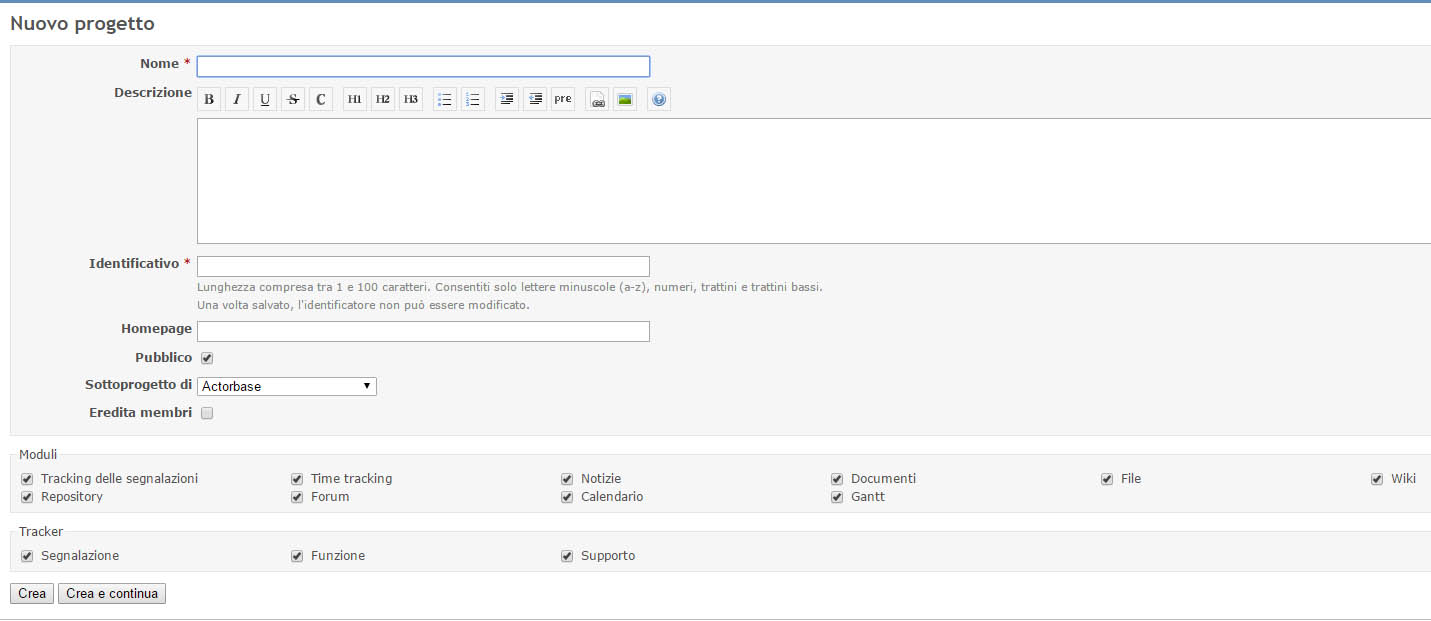
\includegraphics[width=1\textwidth]{tutorialsRedmine/creaproj2.jpg}
  \caption{come creare un sottoprogetto - figura 2\label{fig:figura-2}}
\end{figure}
Come si può vedere in figura \ref{fig:figura-2} si dovrà completare un form con i dati necessari per la creazione del progetto.
\subsection{Scrivere sul Forum}
Si può partecipare al forum rispondendo a messaggi o creandone di nuovi
\subsubsection{Creare un messaggio}
Per creare un nuovo messaggio basta andare nel \gloss{topic} desiderato e seguire la procedura come illustrato nelle seguenti immagini
\begin{figure}[H]
  \centering
  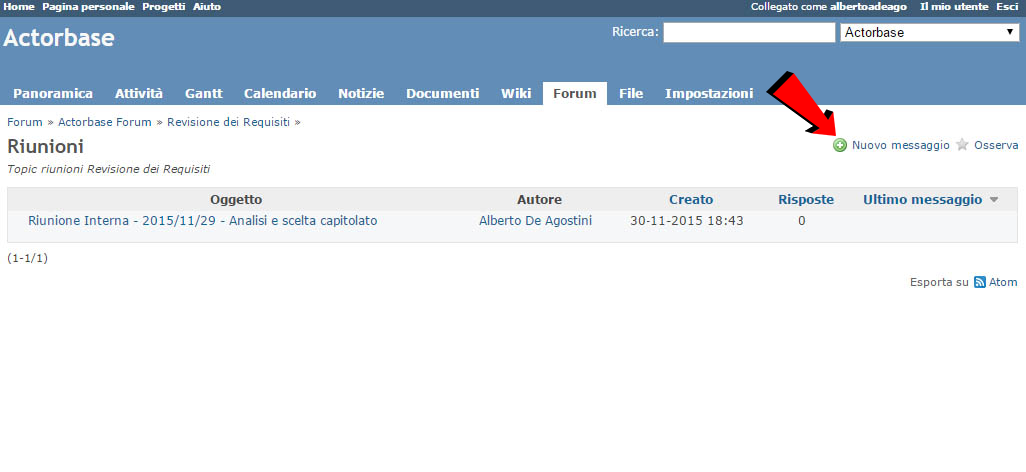
\includegraphics[width=1\textwidth]{tutorialsRedmine/creamessaggio1.png}
  \caption{come creare un messaggio - figura 1}
\end{figure}
\begin{figure}[H]
  \centering
  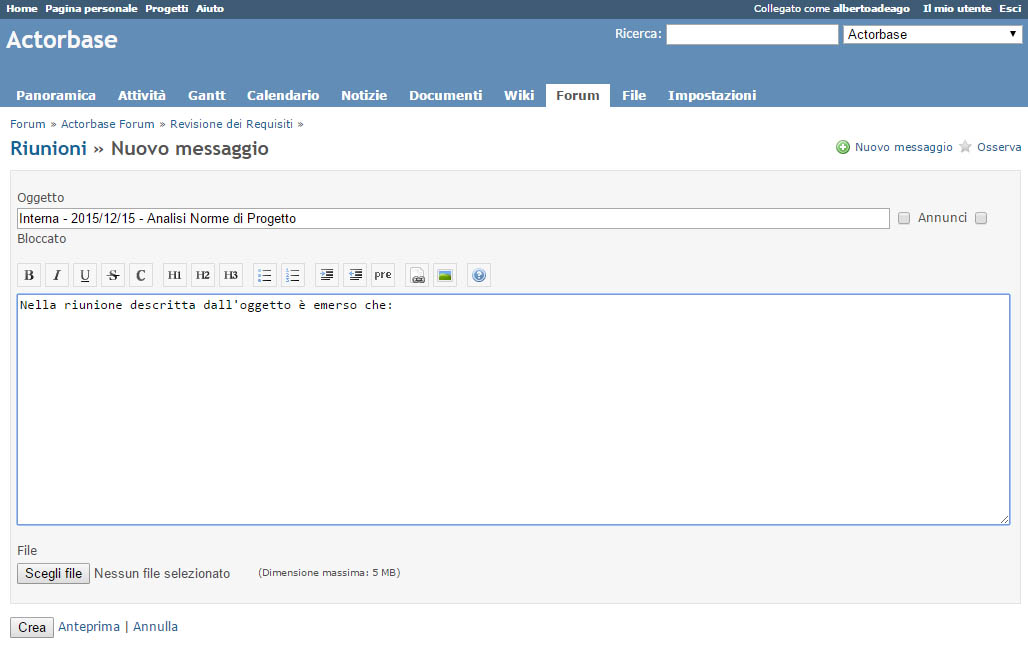
\includegraphics[width=1\textwidth]{tutorialsRedmine/creamessaggio2.jpg}
  \caption{come creare un messaggio - figura 2}
\end{figure}
Per la corretta creazione di un messaggio è necessario seguire le norme scritte nella sezione \ref{sec:Comunicazioni interne}
\subsubsection{Rispondere ad un messaggio}
Per rispondere ad un messaggio presente nel forum è necessario aprire il messaggio voluto e premere su \textbf{Rispondi}, automaticamente ci verrà presentato un form \textit{pre compilato} in cui dovremo solamente inserire il corpo della nostra risposta.
\subsection{Gestione delle segnalazioni}
Una segnalazione rappresenterà una attività che il \textit{Responsabile} assegnerà ad uno o più membri del gruppo, queste attività possono essere suddivise in diverse compiti più semplici da assegnare ad un membro, questi compiti saranno chiamati \gloss{task}.\\
Il sistema di segnalazioni è la cosa più importante di \textit{Redmine}, perciò solamente il \textit{Responsabile di Progetto} ha il potere di creare nuove segnalazioni così da mantenere ordine nel progetto. \\Gli altri membri del gruppo potranno invece aggiornare le segnalazioni assegnate ad essi.
\subsubsection{Creare una segnalazione}
Il \textit{Responsabile di Progetto} può creare nuove segnalazioni facendo come illustrato nelle seguenti immagini
\begin{figure}[H]
  \centering
  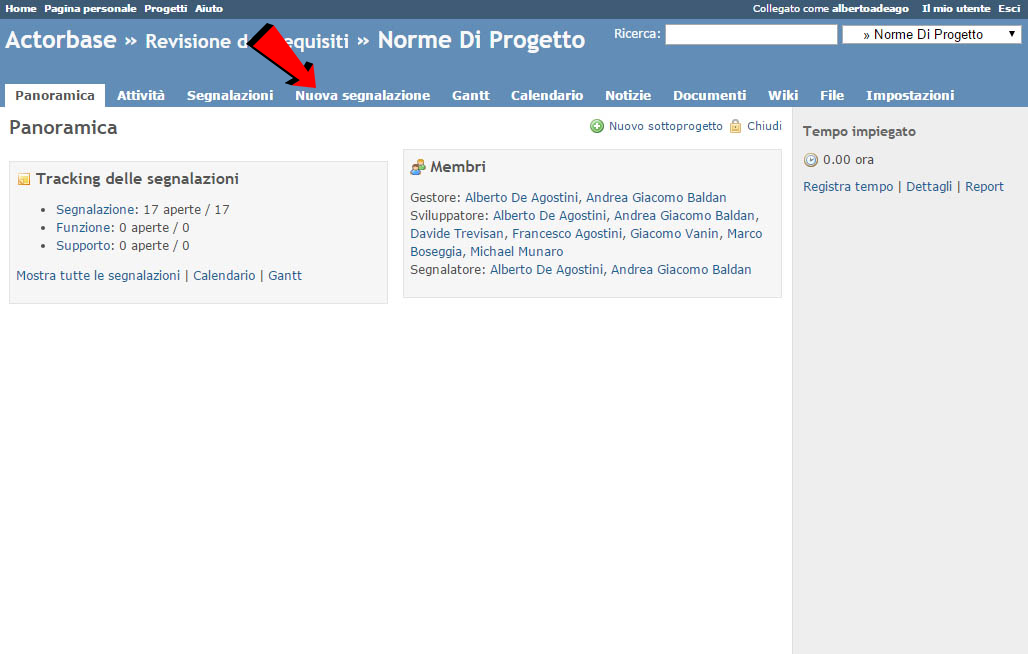
\includegraphics[width=1\textwidth]{tutorialsRedmine/creasegn1.png}
  \caption{come creare un segnalazione - figura 1}
\end{figure}
\begin{figure}[H]
  \centering
  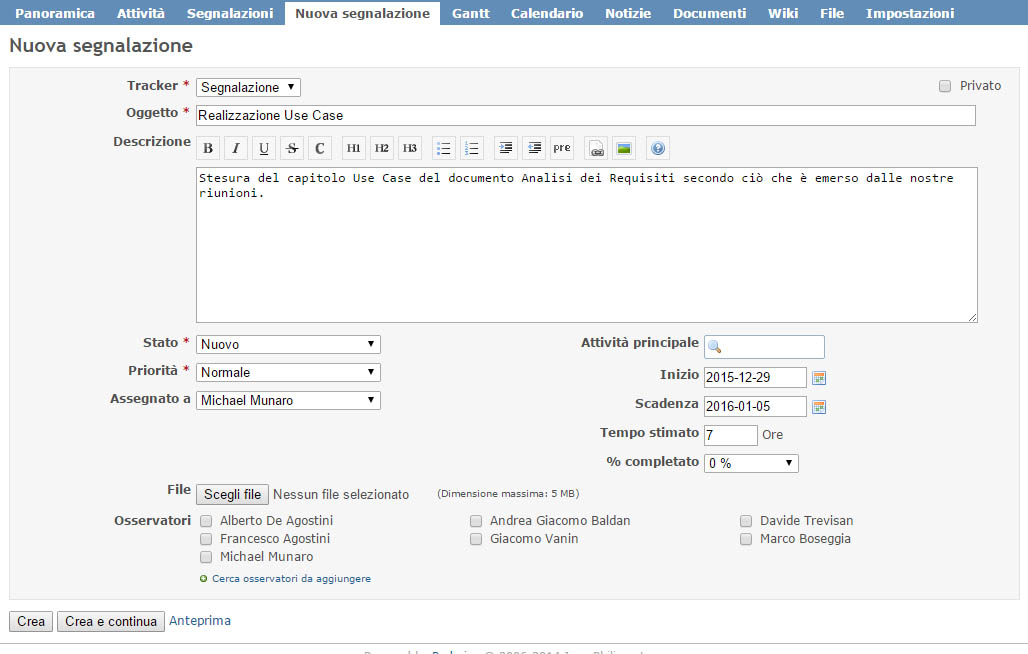
\includegraphics[width=1\textwidth]{tutorialsRedmine/creasegn2.jpg}
  \caption{come creare una segnalazione - figura 2\label{fig:crea-segnalazione-2}}
\end{figure}
Come possiamo vedere in figura \ref{fig:crea-segnalazione-2} ci sono diversi campi da compilare:
\begin{itemize}
  \item \textbf{Tracker:} lasciare selezionato Segnalazione
  \item \textbf{Oggetto:} l'oggetto della segnalazione, questo deve essere breve e non equivocabile
  \item \textbf{Descrizione:} descrizione dettagliata dell'attività da svolgere
  \item \textbf{Stato:} se è una nuova segnalazione deve rimanere \textit{nuovo}, altrimenti è possibile scegliere altre opzioni, di solito lo stato viene cambiato dall'intestatario della segnalazione stessa
  \item \textbf{Assegnato a:} la persona che deve svolgere l'attività
  \item \textbf{Attività principale:} se questa è una sotto \gloss{task} di un altra qui bisogna inserire l'identificatore del \gloss{task} padre
  \item \textbf{Inizio:} data in cui deve iniziare l'attività
  \item \textbf{Fine:} data in cui l'attività deve essere completata
  \item \textbf{Tempo stimato:} il numero di ore stimato in cui si dovrebbe completare questa attività
  \item \textbf{\% completato:} la percentuale di completamento dell'attività, anche questo parametro di solito viene utilizzato dal membro del gruppo che lavora si questa attività.
\end{itemize}
\subsubsection{Aggiornare una segnalazione}
Il lavoro di aggiornamento di una segnalazione deve essere svolto dai vari membri del gruppo che lavorano alla segnalazione stessa.\\
Ad ogni avanzamento fatto relativo ad una attività si deve aggiornare la segnalazione relativa ad essa. Per fare ciò bisogna entrare nella pagina personale di \textit{Redmine} e nella sezione \textbf{Le mie segnalazioni} selezionare la segnalazione desiderata, quindi premere su \textbf{Modifica}.
La schermata che ci si presenterà davanti è come quella descritta in figura \ref{fig:crea-segnalazione-2}, si dovrà quindi aggiornare lo \textbf{stato} (se cambiato), la \textbf{\% completata}, aggiungere inoltre il \textbf{tempo impiegato} e c'è la possibilità di inserire un testo libero, questo può essere utile per spiegare cosa si è fatto.
\subsection{Modificare la Wiki}
La sezione Wiki di \textit{Redmine} può essere molto utile, in pratica è uno spazio in cui si può scrivere del test libero, inserire immagini o altro.\\
Noi abbiamo deciso di usarla come raccoglitore di link a guide inerenti al nostro progetto.
Per contribuire alla nostra Wiki basta solamente andare nella suddetta sezione e premere su \textbf{modifica}. Ci si presenterà un editor di testo in cui è possibile modificare o semplicemente aggiungere del testo.
%TODO: forse solo il responsabile dovrebbe poter modificarla?
%TODO: se uno la cancella?
\end{document}
